ubuntu系统提供了完整的图形化界面，日常操作点点鼠标都能完成。但命令行才是真正的基本功：装环境、连开发板、远程调试，样样绕不开它。下面我们就把最常用的操作过一遍。
\subsubsection{linux文件系统基本概念}
\textbf{linux目录结构}

先看根目录如何把不同用途的文件串成一棵树：

\begin{figure}[H]
    \centering
    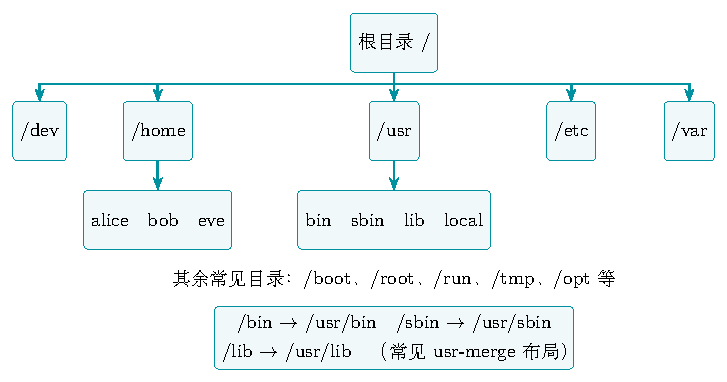
\includegraphics[width=0.9\textwidth]{linux-directory_revised.pdf}
    \caption{Linux 目录树与常见 usr-merge 符号链接} % 图片标题
    \label{fig:linux7} % 图片标签，用于引用
\end{figure}

目录树从根目录 / 出发。图中的 /home 保存用户目录，/usr 保存许多程序与库；在 Ubuntu 的 usr-merge 布局里，/bin、/sbin、/lib 通常是指向 /usr 中对应目录的符号链接，实机可用 ls -ld 检查，不只看图记结论。

\textbf{“一切皆文件”}

在linux系统中有一个非常重要的、区别于windows系统的概念是“一切皆文件”，也就是把一切资源都看作是文件，包括硬件设备（通常称为设备文件），这样好处是用户可以用读写文件的方式实现对硬件的访问。例如 U 盘连接后通常有 /dev 下的块设备节点。对原始设备节点的写入可能破坏分区数据；日常文件操作应使用挂载后的目录，不把设备节点当作普通文本文件。简单来说：你以为是 U 盘设备？其实是我文件哒！

\begin{note}
“一切皆文件”是统一接口的概括，不代表所有资源都是磁盘上的普通文件；设备、管道、套接字有不同类型和操作限制。
\end{note}

\textbf{挂载}

插入 U 盘是连接设备，挂载（Mount）则把某个文件系统接到目录树的一个挂载点上。Linux 当然也有磁盘与分区；只是访问文件时使用统一的目录路径，不按 C:、D: 这样的盘符分树。设备节点如 /dev/sdb1 用来标识分区，挂载点如 /media/alice/USB 用来访问其中的文件，二者不要混淆。

\begin{figure}[H]
    \centering
    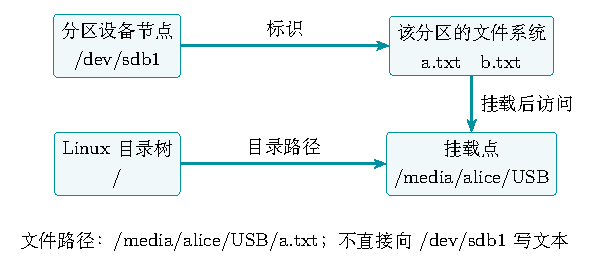
\includegraphics[width=0.85\textwidth]{mount_revised.pdf}
    \caption{把分区中的文件系统接到目录树：设备节点与挂载点各管一层} % 图片标题
    \label{fig:linux8} % 图片标签，用于引用
\end{figure}

Windows的文件系统挂载使用其内部机制完成，用户基本无法探知其过程。而Linux使用mount工具对文件系统进行挂载。挂载文件系统时，需要明确挂载点，在创建文件系统后，操作系统会提示将此文件系统挂载至哪个位置，这个位置就是挂载点，通常U盘等设备系统会自动挂载到“/media”目录下。挂载操作在备份系统镜像时经常用到。

\textbf{主要文件夹及其作用}

/bin：bin 是 Binaries (二进制文件) 的缩写, 这个目录存放着最经常使用的命令。

/boot：这里存放的是启动 Linux 时使用的一些核心文件，包括一些连接文件以及镜像文件。

/dev：dev 是 Device(设备) 的缩写, 该目录下存放的是 Linux 的外部设备，在 Linux 中访问设备的方式和访问文件的方式是相同的。

/etc：etc 是 Etcetera(等等) 的缩写,这个目录用来存放所有的系统管理所需要的配置文件和子目录。

/home：用户的主目录，在 Linux 中，每个用户都有一个自己的目录，一般该目录名是以用户的账号命名的，例如 alice、bob 和 eve。

/lib：lib 是 Library(库) 的缩写这个目录里存放着系统最基本的动态连接共享库，其作用类似于 Windows 里的 DLL 文件。几乎所有的应用程序都需要用到这些共享库。

/opt：常用于放额外安装的软件，是否为空取决于本机安装情况。

/root：该目录为系统管理员，也称作超级权限者的用户主目录。

/usr：保存许多程序、库和共享数据；不是普通用户的个人资料目录，个人文件通常放在 /home/用户名。

/var：var 是 variable(变量) 的缩写，这个目录中存放着在不断扩充着的东西，我们习惯将那些经常被修改的目录放在这个目录下。包括各种日志文件。

在这些文件夹中，绝大多数目录都包含重要的系统文件，如果随意删除可能会导致系统出错，因此在平时操作时要多加注意。

\Needspace{8\baselineskip}
\begin{example}[查看目录、设备和挂载点]


\Needspace{8\baselineskip}
\begin{tbash}
ls /
ls -ld /bin /usr/bin
ls -l /dev/null /dev/zero
findmnt /
\end{tbash}


目录类型以 d 开头，符号链接以 l 开头，字符设备以 c 开头；findmnt 显示根目录对应的文件系统。设备文件不是可随意删除的普通文件。
\end{example}
\begin{exercise}\label{ex:v1-fs-layout}
在终端执行 \texttt{ls /} 查看根目录下的文件夹，对照本节内容说出 \texttt{/etc}、\texttt{/home}、\texttt{/dev} 各自的作用；再执行 \texttt{ls /dev}，找出其中的设备文件。
\end{exercise}

\subsubsection{linux系统基本操作}
由于篇幅有限，本部分仅能列出平时操作中最常用的部分，其它内容如需用到请读者自行查阅资料。

\textbf{01用户管理}
\begin{table}[!htbp]
	\centering
	\begin{tabular}{p{0.40\textwidth}p{0.51\textwidth}}
		\toprule[1.5pt]
		命令 & 作用\\
		\midrule[1pt]
		\texttt{id   [name]}			&查看用户UID和GID信息\\
		\texttt{who}			&查看当前所有登录的用户列表\\
		\texttt{whoami}			&查看当前登录用户的账户名\\
		\texttt{su   -   [name]}			&切换用户，并且切换目录\\
		\texttt{exit}			&退出当前登录用户\\
		\texttt{passwd  [name]}			&设置用户密码\\
		\bottomrule[1.5pt]
	\end{tabular}
\end{table}

说明：
\begin{enumerate}
	\item -\enspace 可以切换到用户家目录，否则保持位置不变
	\item su 不接用户名通常尝试切换到 root；Ubuntu 默认不启用 root 密码，日常管理员命令用 sudo，不为练习开启 root 登录
	\item 命令前加sudo：以超级用户权限运行命令
\end{enumerate}

\Needspace{8\baselineskip}
\begin{example}
查看当前登录用户的账户名与 UID/GID 信息：


\Needspace{6\baselineskip}
\begin{tbash}
whoami
id
\end{tbash}


\end{example}

\begin{exercise}\label{ex:v1-user-info}
用 whoami 与 id 记录当前用户名、UID、主组和附加组，说明为什么“命令加 sudo”不等于“桌面用户永久变成 root”。
\end{exercise}
\textbf{02系统信息}

\begin{table}[!htbp]
	\centering
	\begin{tabular}{p{0.40\textwidth}p{0.51\textwidth}}
		\toprule[1.5pt]
		语法 & 作用\\
		\midrule[1pt]
		\texttt{free  [options]}			&显示系统内存使用情况\\
		\texttt{uname  [options]}			&显示电脑以及操作系统的相关信息\\
		\texttt{df  [options]  [file]}			&显示文件系统的磁盘空间使用情况\\
		\texttt{du  [options]  [directory]}			&显示目录或文件的磁盘占用量\\
		\texttt{top}			&动态显示系统中运行的进程及资源占用情况\\
		\texttt{hostname}			&查看当前主机名\\
		\bottomrule[1.5pt]
	\end{tabular}
\end{table}


\begin{table}[H]\centering
\textbf{free\enspace 选项和参数}

	\begin{tabular}{p{0.40\textwidth}p{0.51\textwidth}}
		\toprule[1.5pt]
		参数 & 作用\\
		\midrule[1pt]
		\texttt{-h}		&以易读的单位（GiB、MiB 等）显示\\
		\texttt{-m}		&以 MiB 为单位显示\\
		\texttt{-g}		&以 GiB 为单位显示\\
		\texttt{-s}\enspace [秒数] 		&每隔指定秒数持续刷新显示\\
		\bottomrule[1.5pt]
	\end{tabular}
\end{table}



\begin{table}[H]\centering
\textbf{uname\enspace 选项和参数}

	\begin{tabular}{p{0.40\textwidth}p{0.51\textwidth}}
		\toprule[1.5pt]
		参数 & 作用\\
		\midrule[1pt]
		\texttt{-a  --all}		&显示全部的信息\\
		\texttt{-m  --machine}		&显示处理器类型\\
		\texttt{-n  --nodename}		&显示主机名\\
		\texttt{-r  --release}		&显示内核版本号\\
		\texttt{-s  --sysname}		&显示操作系统名称\\
		\texttt{-v}		&显示内核构建版本信息\\
		\texttt{--help}		&显示帮助\\
		\texttt{--version}		&显示版本信息\\
		\texttt{-p}		&显示处理器信息，可能为 unknown，不保证与 -m 相同\\
		\bottomrule[1.5pt]
	\end{tabular}
\end{table}



\begin{table}[H]\centering
\textbf{df\enspace 选项和参数}

	\begin{tabular}{p{0.40\textwidth}p{0.51\textwidth}}
		\toprule[1.5pt]
		参数 & 作用\\
		\midrule[1pt]
		\texttt{-h}		&以易读的单位（GiB、MiB 等）显示\\
		\texttt{-T}		&同时显示文件系统类型\\
		\bottomrule[1.5pt]
	\end{tabular}
\end{table}



\begin{table}[H]\centering
\textbf{du\enspace 选项和参数}

	\begin{tabular}{p{0.40\textwidth}p{0.51\textwidth}}
		\toprule[1.5pt]
		参数 & 作用\\
		\midrule[1pt]
		\texttt{-h}		&以易读的单位（GiB、MiB 等）显示\\
		\texttt{-s}		&只显示总计，不列出每个子目录\\
		\texttt{--max-depth=1}		&只统计指定层级的子目录\\
		\bottomrule[1.5pt]
	\end{tabular}
\end{table}


你可以用 man 命令查阅完全的参数详情（例如\texttt{man du}查询du命令的全体参数）。

\Needspace{8\baselineskip}
\begin{example}
统计当前目录下各子目录的磁盘占用，并按易读单位显示：


\Needspace{5\baselineskip}
\begin{tbash}
du -h --max-depth=1 .
\end{tbash}


\end{example}

\Needspace{8\baselineskip}
\begin{example}[区分内存、磁盘与目录占用]


\Needspace{9\baselineskip}
\begin{tbash}
free -h
uname -r
hostname
df -hT /
du -h --max-depth=1 .
\end{tbash}


free 的 available 估计当前可用内存，df 描述根文件系统容量，du 累计当前目录文件占用。它们不是同一个“还剩多少”。
\end{example}
\begin{exercise}\label{ex:v1-disk-space}
执行 \texttt{df -hT} 查看各文件系统的磁盘使用情况，找到你的根分区（挂载点为 \texttt{/} 的一行），记录其文件系统类型、容量与已用空间；再记录 free 的 available 和 uname 的内核版本，说明这些值与磁盘容量的差别。
\end{exercise}

\textbf{03软件安装}

软件安装命令有apt，snap，yum等等，在我们ubuntu系统中用的是apt，不过有时候也得用到snap。安装和卸载软件需要root权限。

\begin{table}[!htbp]
	\centering
	\begin{tabular}{p{0.40\textwidth}p{0.51\textwidth}}
		\toprule[1.5pt]
		语法 & 作用\\
		\midrule[1pt]
		\texttt{apt  [options]   [command]   [package ...]}		&查找、安装、升级、删除软件包\\
		\bottomrule[1.5pt]
	\end{tabular}
\end{table}

\textbf{options}：可选，选项包括 -h（帮助），-y（当安装过程提示选择全部为"yes"），-q（不显示安装的过程）等等

\textbf{command}：要进行的操作

\textbf{package}：安装的包名\\


\begin{table}[H]\centering
\textbf{apt常用命令如下}

	\begin{tabular}{p{0.40\textwidth}p{0.51\textwidth}}
		\toprule[1.5pt]
		命令 & 作用\\
		\midrule[1pt]
		\texttt{apt  update}	&刷新软件包索引，不会升级已安装包\\
		\texttt{apt  upgrade}	&升级软件包\\
		\texttt{apt  list   --upgradable}		&列出可更新的软件包及版本信息\\
		\texttt{apt  full-upgrade}	&处理依赖变化的升级，可能移除包，先读变更清单\\
		\texttt{apt  install   \textless package1\textgreater   \textless package2\textgreater}	&安装指定的软件\\
		\texttt{apt  install   --only-upgrade  \textless package\textgreater}		&更新指定的软件\\
		\texttt{apt  show   \textless package\textgreater}	&显示软件包具体信息\\
		\texttt{apt  remove   \textless package\textgreater}		&删除软件包\\
		\texttt{apt  autoremove}		&清理不再使用的依赖和库文件\\
		\texttt{apt  purge \textless package\textgreater}		&移除软件包及配置文件\\
		\texttt{apt  search   \textless keyword\textgreater}		&找软件包命令\\
		\texttt{apt  list   --installed}		&列出所有已安装的包\\
		\texttt{apt  list   --all-versions}	&列出包索引中可用的各版本\\
		\bottomrule[1.5pt]
	\end{tabular}
\end{table}


与上文类似，其余命令与参数请查阅 man 手册（\texttt{man apt}）。

\Needspace{8\baselineskip}
\begin{example}
更新软件清单后安装 \texttt{tree}（一个以树状图显示目录结构的小工具）：


\Needspace{6\baselineskip}
\begin{tbash}
sudo apt update
sudo apt install tree
\end{tbash}


\end{example}

\begin{exercise}\label{ex:v1-apt-package}
使用 \texttt{apt search} 搜索并安装一个你感兴趣的小软件（如 \texttt{cowsay}），运行验证后用 \texttt{sudo apt remove} 将其卸载。
\end{exercise}

\textbf{04文件与目录管理}

先认识几个常用概念，后面的命令都要用到它们：

\begin{enumerate}
\item 绝对路径：路径的写法，由根目录\enspace /\enspace 写起，例如：/usr/share/doc 这个目录。
\item 相对路径：路径的写法，相对于当前所处的文件夹位置，不是由\enspace /\enspace 写起，例如由 /usr/share/doc 要到 /usr/share/man，可以写成：cd ../man
\item \enspace .\enspace ：表示当前目录
\item \enspace ..\enspace ：表示上一级目录
\item 文件类型：分为目录（d），文件（-），链接文件（l），装置文件里可供储存的接口设备（b），字符设备（c，例如终端、串口、/dev/null）
\item 文件基本属性：分为可读（r），可写（w），可执行（x）。Linux文件属性有两种设置方法，一种是数字，一种是符号。使用数字来代表各个权限时，各权限的分数对照为：r:4，w:2，x:1
\item 文件所有者（user）：表示该文件或目录的拥有者，也就是文件权限中的第一个权限对象（u）。
\item 用户组（group）：表示该文件或目录所属的用户组，也就是文件权限中的第二个权限对象（g）。文件权限通常依次针对文件所有者、所属用户组以及其他用户（others）进行设置。
\item 其他用户（others）：表示既不是文件所有者，也不属于该文件所属用户组的其他用户，是文件权限中的第三个权限对象（o）。
\item 路径名展开（pathname expansion）：属于 Shell（如 Bash）的语法，用于使用通配符匹配文件名。常见的通配符包括 \enspace * \enspace、\enspace ? \enspace 和 \enspace [ ] \enspace。例如：\enspace *.txt \enspace 可以匹配当前目录下所有以 .txt 结尾的文件；\enspace ? \enspace 表示匹配一个字符；\enspace [abc] \enspace 表示匹配 a、b 或 c 中的一个字符。
\end{enumerate}

处理文件和目录的命令有很多，这里分表整理了一些常用命令的语法及其选项和参数仅供大家参考


\begin{table}[H]\centering
\textbf{常用处理文件和目录的命令}

	\begin{tabular}{p{0.40\textwidth}p{0.51\textwidth}}
		\toprule[1.5pt]
		语法 & 作用\\
		\midrule[1pt]
		\texttt{ls}		&列出当前目录中的文件和子目录\\
		\texttt{pwd}		&显示当前工作目录的路径\\
		\texttt{cd  /path/to/directory}		&切换工作目录\\
		\texttt{mkdir  [directory]}		&创建新目录\\
		\texttt{cp  [source]  [destination]}		&复制文件或目录\\
		\texttt{rm  [file name]}		&删除文件或目录\\
		\texttt{mv  [old]  [new]}		&移动或重命名文件或目录\\
		\texttt{ln  [options]  [source]  [link name]}		&创建链接文件\\
		\texttt{chmod  [permissions]  [file name]}		&修改文件或目录的权限\\
		\texttt{tar  [options]  -f  archive.tar  [files...]}	&解压或压缩文件或目录\\
		\texttt{zip  [options]  output.zip  [files...]}		&压缩文件或目录\\
		\texttt{unzip  archive.zip}		&解压文件或目录\\
		\bottomrule[1.5pt]
	\end{tabular}
\end{table}



\begin{table}[H]\centering
\textbf{ls\enspace 选项和参数}

	\begin{tabular}{p{0.40\textwidth}p{0.51\textwidth}}
		\toprule[1.5pt]
		参数 & 作用\\
		\midrule[1pt]
		\texttt{-a}		&列出当前目录中全部的文件，包括隐藏文件\\
		\texttt{-d}		&仅列出目录本身，而不是列出目录内的文件数据\\
		\texttt{-l}		&长数据串列出，包含文件的属性与权限等\\
		\bottomrule[1.5pt]
	\end{tabular}
\end{table}



\begin{table}[H]\centering
\textbf{mkdir\enspace 选项和参数}

	\begin{tabular}{p{0.40\textwidth}p{0.51\textwidth}}
		\toprule[1.5pt]
		参数 & 作用\\
		\midrule[1pt]
		\texttt{-m}		&配置文件的权限\\
		\texttt{-p}		&递归创建所需目录\\
		\bottomrule[1.5pt]
	\end{tabular}
\end{table}



\begin{table}[H]\centering
\textbf{cp\enspace 选项和参数}

	\begin{tabular}{p{0.40\textwidth}p{0.51\textwidth}}
		\toprule[1.5pt]
		参数 & 作用\\
		\midrule[1pt]
		\texttt{-a}		&相当于\enspace -pdr\enspace 的意思\\
		\texttt{-d}		&若来源档为链接档的属性(link file)，则复制链接档属性而非文件本身\\
		\texttt{-f}		&强制，若目标文件已经存在且无法开启，则移除后再尝试一次\\
		\texttt{-i}		&若目标文件或目录已经存在，在覆盖时会先询问用户\\
		\texttt{-l}		&进行硬式链接的链接档创建，而非复制文件本身\\
		\texttt{-p}		&连同文件的属性一起复制过去，而非使用默认属性(备份常用)\\
		\texttt{-r}		&递归持续复制，用于目录的复制(常用)\\
		\texttt{-s}		&复制成为符号链接档，即“捷径”文件\\
		\texttt{-u}		&若 destination 比 source 旧才升级 destination\\
		\bottomrule[1.5pt]
	\end{tabular}
\end{table}



\begin{table}[H]\centering
\textbf{rm\enspace 选项和参数}

	\begin{tabular}{p{0.40\textwidth}p{0.51\textwidth}}
		\toprule[1.5pt]
		参数 & 作用\\
		\midrule[1pt]
		\texttt{-f}		&强制的意思，删除时不询问且忽略不存在的文件\\
		\texttt{-i}		&互动模式，在删除前会询问使用者是否动作\\
		\texttt{-r}		&递归删除,常用在目录的删除\\
		\bottomrule[1.5pt]
	\end{tabular}
\end{table}


\begin{note}
\texttt{rm -rf} 会不做任何确认地递归删除目标及其全部内容，且命令行下的删除不进回收站，无法恢复。这条命令删库跑路一气呵成，使用前请三思——你的存档没有读档功能。脚本中使用 \texttt{rm -rf \$dir/} 这类写法时，务必先检查变量非空：变量一旦为空，路径可能直接变成根目录。
\end{note}


\begin{table}[H]\centering
\textbf{mv\enspace 选项和参数}

	\begin{tabular}{p{0.40\textwidth}p{0.51\textwidth}}
		\toprule[1.5pt]
		参数 & 作用\\
		\midrule[1pt]
		\texttt{-f}		&强制的意思，如果目标文件已经存在，不会询问而直接覆盖\\
		\texttt{-i}		&若目标文件已经存在时，会询问是否覆盖\\
		\texttt{-u}		&若目标文件已经存在，且 source 比较新，才会升级 \\
		\bottomrule[1.5pt]
	\end{tabular}
\end{table}



\begin{table}[H]\centering
\textbf{ln\enspace 选项和参数}

	\begin{tabular}{p{0.40\textwidth}p{0.51\textwidth}}
		\toprule[1.5pt]
		参数 & 作用\\
		\midrule[1pt]
		\texttt{-s}		&创建符号链接（软链接），不加该选项时默认创建硬链接\\
		\texttt{-f}		&强制创建，若链接文件已存在则直接覆盖\\
		\bottomrule[1.5pt]
	\end{tabular}
\end{table}


\begin{conclusion}
硬链接、软链接与复制的区别：

\begin{itemize}
\item 硬链接：与源文件指向同一份数据，删除源文件不影响链接；但不能跨文件系统，也不能给目录创建；
\item 软链接（符号链接）：类似 Windows 的快捷方式，只记录源文件的路径；源文件被删除后链接失效，但可以跨文件系统、可以链接目录；
\item 复制（cp）：得到一份完全独立的新文件，与源文件互不影响。
\end{itemize}
\end{conclusion}


\begin{table}[H]\centering
\textbf{chmod\enspace 选项和参数}

	\begin{tabular}{p{0.40\textwidth}p{0.51\textwidth}}
		\toprule[1.5pt]
		参数 & 作用\\
		\midrule[1pt]
		\texttt{-R}		&进行递归的持续变更，连同次目录下的所有文件都会变更\\
		\texttt{u}		&user，用户身份\\
		\texttt{g}		&group，组 \\
		\texttt{o}		&others，其他身份 \\
		\texttt{a}		&all，全部的身份 \\
		\texttt{+  -  =}		&对权限加入，除去，设定 \\
		\bottomrule[1.5pt]
	\end{tabular}
\end{table}


使用chmod命令修改文件或目录权限有两种方式。一是用数字类型的权限属性更改，通用形式为：

chmod\enspace [-R]\enspace xyz\enspace 文件或目录

其中 xyz 是三位数字，分别对应所有者、用户组、其他用户的权限，每位数字为该身份 rwx 属性数值（r:4，w:2，x:1）的和。二是用符号类型改变文件权限，通用形式为：

chmod\enspace [身份]\enspace +/-/=\enspace [permissions]\enspace [file name]

\Needspace{8\baselineskip}
\begin{example}
先在独立练习目录创建两个空文件，再只给脚本所需权限：


\Needspace{8\baselineskip}
\begin{tbash}
touch ex1.py run.sh
chmod u+x ex1.py
chmod 755 run.sh
ls -l ex1.py run.sh
\end{tbash}


\end{example}

\begin{note}
不要图省事对所有文件都 \texttt{chmod 777}——这相当于把家门钥匙挂在门外，谁路过都能进来逛一圈。权限放得越宽，误操作和恶意篡改的风险越大；脚本只需要给所有者加上执行权限（\texttt{chmod u+x}）就够了。
\end{note}

\begin{exercise}\label{ex:v1-file-ops}
在家目录下创建 \texttt{practice} 目录，在其中新建文件 \texttt{hello.txt}，将它复制为 \texttt{hello\_bak.txt}，再把原文件移动到 \texttt{practice/sub} 目录（该目录需用 \texttt{mkdir} 一并创建），最后删除整个 \texttt{practice} 目录。
\end{exercise}


\begin{table}[H]\centering
\textbf{tar\enspace 选项和参数}

	\begin{tabular}{p{0.40\textwidth}p{0.51\textwidth}}
		\toprule[1.5pt]
		参数 & 作用\\
		\midrule[1pt]
		\texttt{-c}		&创建新的归档文件\\
		\texttt{-f}		&指定归档文件的名称\\
		\texttt{-v}		&显示详细输出，列出被添加/解压到归档中的文件 \\
		\texttt{-x}		&解压归档文件 \\
		\texttt{-z}		&使用 gzip 压缩归档文件 \\
		\texttt{-r}		&向已存在的归档中追加文件 \\
		\bottomrule[1.5pt]
	\end{tabular}
\end{table}


tar命令的参数繁多，此处只列举了以上最最常见的参数。


\begin{table}[H]\centering
\begin{note}
归档命令也有删除选项：zip 的 -m 会在压缩后移除源文件，本章练习不使用它；tar 的 -r 只适用于可追加的未压缩归档，不直接追加到 .tar.gz。先保留源数据，再做解包核验。
\end{note}
\textbf{zip\enspace 选项和参数}

	\begin{tabular}{p{0.40\textwidth}p{0.51\textwidth}}
		\toprule[1.5pt]
		参数 & 作用\\
		\midrule[1pt]
		\texttt{-r}		&递归压缩目录及其子目录中的所有文件\\
		\texttt{-e}		&为压缩文件设置密码保护\\
		\texttt{-q}		&静默模式，不显示压缩过程 \\
		\texttt{-v}		&显示详细的压缩过程 \\
		\texttt{-x}		&排除某些文件或目录，不进行压缩 \\
		\texttt{-m}		&压缩后删除原始文件 \\
		\texttt{-0}\enspace \textasciitilde\enspace \texttt{-9}		&指定压缩级别，-0 表示存储不压缩，-9 表示最高压缩率，默认是 -6 \\
		\bottomrule[1.5pt]
	\end{tabular}
\end{table}


\Needspace{8\baselineskip}
\begin{example}[硬链接、软链接和复制]
在新练习目录中执行，不改真实资料：


\Needspace{11\baselineskip}
\begin{tbash}
printf 'armor\n' > original.txt
ln original.txt hard.txt
ln -s original.txt soft.txt
cp original.txt copy.txt
printf 'radar\n' >> original.txt
ls -li original.txt hard.txt soft.txt copy.txt
cat hard.txt copy.txt
\end{tbash}


原文件与硬链接 inode 相同，内容一起变化；复制件仍只有 armor，软链接保存路径。先不删除文件，用这份状态对照前面的归纳。
\end{example}
\begin{exercise}\label{ex:v1-links-permissions-archive}
在独立目录复现链接例题，给一个练习脚本设置 755，记录 ls -l 与 ls -i。把目录打包，再解到新的空目录并比较内容。说明链接、复制、权限和归档各解决什么问题，不对设备文件 chmod 777。
\end{exercise}
\textbf{05查找、管道与重定向}


\begin{table}[H]\centering
\textbf{find\enspace 的语法}

	\begin{tabular}{p{0.40\textwidth}p{0.51\textwidth}}
		\toprule[1.5pt]
		语法 & 作用\\
		\midrule[1pt]
		\texttt{find  [path]  [option]  [expression]}		&在指定目录下查找符合条件的文件或目录\\
		\bottomrule[1.5pt]
	\end{tabular}
\end{table}


\textbf{path}：要查找的起始目录，省略时默认从当前目录开始查找

\textbf{expression}：查找条件，例如文件名、文件类型等\\


\begin{table}[H]\centering
\textbf{find\enspace 的参数}

	\begin{tabular}{p{0.40\textwidth}p{0.51\textwidth}}
		\toprule[1.5pt]
		参数 & 作用\\
		\midrule[1pt]
		\texttt{-name  pattern}		&按文件名查找，支持通配符\\
		\texttt{-iname  pattern}		&按文件名查找，忽略大小写\\
		\texttt{-type  f/d/l}		&按类型查找，f 为普通文件，d 为目录，l 为链接文件\\
		\texttt{-size  [+/-]n}		&按文件大小查找，+ 表示大于，- 表示小于\\
		\texttt{-mtime  [+/-]n}		&按修改时间查找，n 表示 n 天前\\
		\bottomrule[1.5pt]
	\end{tabular}
\end{table}


其余参数请查阅 man 手册（\texttt{man find}）。

\Needspace{8\baselineskip}
\begin{example}
先在练习目录建样本，再查找自己的文件，避免其他用户目录的权限错误干扰判断：


\Needspace{8\baselineskip}
\begin{tbash}
mkdir -p test
touch test/hello.txt
find . -type f -name "*.txt"
find . -type d -name "test"
\end{tbash}


\end{example}


\begin{table}[H]\centering
\textbf{grep\enspace 的语法}

	\begin{tabular}{p{0.40\textwidth}p{0.51\textwidth}}
		\toprule[1.5pt]
		语法 & 作用\\
		\midrule[1pt]
		\texttt{grep  [option]  pattern  [files]}		&查找文件里符合条件的字符串或正则表达式\\
		\bottomrule[1.5pt]
	\end{tabular}
\end{table}


\textbf{pattern}：表示要查找的字符串或正则表达式

\textbf{files}：要查找的文件名，可以同时查找多个文件，如果省略 files 参数，则默认从标准输入中读取数据\\

重定向是一种强大的功能，它允许用户改变命令的输入或输出方向，从而更灵活地控制数据流。重定向主要包括三种类型：标准输入重定向(stdin)、标准输出重定向（stdout）和标准错误输出重定向（stderr）。


\begin{table}[H]\centering
\textbf{重定向}

	\begin{tabular}{p{0.13\textwidth}p{0.22\textwidth}p{0.54\textwidth}}
		\toprule[1.5pt]
		输入输出 & 重定向 & 意义\\
		\midrule[1pt]
		\texttt{stdin}		& <\enspace /\enspace <<		& <从文件读取内容作为命令的输入，<<以指定字符串作为输入的结束标志\\
		\texttt{stdout}		& >\enspace /\enspace >>		& >会覆盖文件原有内容，>>则会在文件末尾追加内容\\
		\texttt{stderr}		& 2>\enspace /\enspace 2>>		&作用与标准输出重定向类似，但专门用于处理错误信息\\
		\bottomrule[1.5pt]
	\end{tabular}
\end{table}


管道符|主要用于多重命令处理，前面命令的打印结果作为后面命令的输入,不过其默认连接标准输出；失败的命令也可能有标准输出，成功的命令也可能写标准错误

管道符常和grep结合使用用于过滤信息，列出所查找关键字所在的位置


\begin{table}[H]\centering
\textbf{grep的参数}

	\begin{tabular}{p{0.40\textwidth}p{0.51\textwidth}}
		\toprule[1.5pt]
		参数 & 作用\\
		\midrule[1pt]
		\texttt{-i}		&忽略大小写进行匹配\\
		\texttt{-v}		&反向查找，只打印不匹配的行\\
		\texttt{-n}		&显示匹配行的行号\\
		\texttt{-r}		&递归查找子目录中的文件\\
		\texttt{-l}		&只打印匹配的文件名\\
		\texttt{-c}		&只打印匹配的行数\\
		\bottomrule[1.5pt]
	\end{tabular}
\end{table}


其余参数请查阅 man 手册（\texttt{man grep}）。

\Needspace{8\baselineskip}
\begin{example}
内核日志在部分机器上需要权限。先用自带样本观察 grep 的筛选与行号，再用于真实日志：


\Needspace{7\baselineskip}
\begin{tbash}
printf 'ok\nerror: sample\nok\n' > sample.log
grep -n error sample.log
cat sample.log | grep -n error
\end{tbash}


\end{example}

\Needspace{8\baselineskip}
\begin{example}[把筛选结果写入新文件]


\Needspace{8\baselineskip}
\begin{tbash}
grep -n error sample.log > errors.txt
printf 'checked\n' >> errors.txt
cat errors.txt
wc -l < errors.txt
\end{tbash}


应显示 2:error: sample 与 checked，共两行。大于号先截断目标文件，两个大于号追加，输入重定向把文件内容交给 wc；普通管道默认只传标准输出。
\end{example}
\begin{exercise}\label{ex:v1-find-python}
使用 find 在你的家目录下查找所有 7 天内修改过的 \texttt{.py} 文件。
\end{exercise}

\begin{exercise}\label{ex:v1-pipe-count}
使用管道和 grep，从 \texttt{apt list --installed} 的输出中筛选出名字包含 \texttt{python} 的软件包；再结合 \texttt{wc -l} 统计数量；将筛选结果重定向到新文件，再读取该文件统计行数并核对一致。
\end{exercise}

\textbf{06文件内容}


\begin{table}[H]\centering
\textbf{文件内容操作}

	\begin{tabular}{p{0.40\textwidth}p{0.51\textwidth}}
		\toprule[1.5pt]
		语法 & 作用\\
		\midrule[1pt]
		\texttt{cat [file name]}		&由第一行开始显示文件内容（只读）\\
		\texttt{head [file name]}		&显示文件开头的内容（默认前10行）\\
		\texttt{tail [file name]}		&显示文件末尾的内容（默认后10行）\\
		\texttt{less [file name]}		&分页查看文件内容，可上下翻页，按 q 退出\\
		\texttt{touch [file name]}		&创建空文件或更新文件的时间戳\\
		\texttt{gedit [file name]}		&创建空文件或更改文件内容\\
		\texttt{vim/vi [file name]}		&创建空文件或编辑文件内容\\
		\bottomrule[1.5pt]
	\end{tabular}
\end{table}



\begin{table}[H]\centering
\textbf{head/tail\enspace 选项和参数}

	\begin{tabular}{p{0.40\textwidth}p{0.51\textwidth}}
		\toprule[1.5pt]
		参数 & 作用\\
		\midrule[1pt]
		\texttt{-n}\enspace [行数] 		&指定显示的行数（head 与 tail 均适用）\\
		\texttt{-f}		&（仅 tail）持续跟踪文件末尾的新增内容，常用于查看日志\\
		\bottomrule[1.5pt]
	\end{tabular}
\end{table}


在所有关于文件内容的操作中，这里着重介绍一下vim。vim是从 vi 发展出来的一个文本编辑器。代码补全、编译及错误跳转等方便编程的功能特别丰富。

vi/vim 共分为三种模式，命令模式、输入模式和命令行模式

\textbf{命令模式}：用户刚刚启动 vi/vim，便进入了命令模式。此状态下敲击键盘动作会被 vim 识别为命令，而非输入字符，比如我们此时按下i，并不会输入一个字符，i被当作了一个命令。


\begin{table}[H]\centering
\textbf{命令模式常用操作}

	\begin{tabular}{p{0.40\textwidth}p{0.51\textwidth}}
		\toprule[1.5pt]
		命令 & 作用\\
		\midrule[1pt]
		\texttt{i}		&切换到输入模式，在光标当前位置开始输入文本\\
		\texttt{x}		&删除当前光标所在处的字符\\
		\texttt{:}		&切换到底线命令模式，以在最底一行输入命令\\
		\texttt{a}		&进入插入模式，在光标下一个位置开始输入文本\\
		\texttt{o}		&在当前行的下方插入一个新行，并进入插入模式\\
		\texttt{O}		&在当前行的上方插入一个新行，并进入插入模式\\
		\texttt{dd}		&剪切当前行\\
		\texttt{yy}		&复制当前行\\
		\texttt{p}		&粘贴剪贴板内容到光标下方\\
		\texttt{P}		&粘贴剪贴板内容到光标上方\\
		\texttt{u}		&撤销上一次操作\\
		\texttt{Ctrl + r}		&重做上一次撤销的操作\\
		\bottomrule[1.5pt]
	\end{tabular}
\end{table}


\textbf{输入模式}：在此状态下敲击键盘会被vim识别为输入内容，同时也有一些按键命令。


\begin{table}[H]\centering
\textbf{输入模式常用操作}

	\begin{tabular}{p{0.40\textwidth}p{0.51\textwidth}}
		\toprule[1.5pt]
		命令 & 作用\\
		\midrule[1pt]
		\texttt{keyboard+Shift}		&输入字符\\
		\texttt{ENTER}		&回车键，换行\\
		\texttt{BACK SPACE}		&退格键，删除光标前一个字符\\
		\texttt{DEL}		&删除键，删除光标后一个字符\\
		\texttt{Arrow keys}		&在文本中移动光标\\
		\texttt{HOME/END}		&移动光标到行首/行尾\\
		\texttt{Page Up/Page Down}		&上/下翻页\\
		\texttt{Insert}		&切换光标为输入/替换模式，光标将变成竖线/下划线\\
		\texttt{ESC}		&退出输入模式，切换到命令模式\\
		\bottomrule[1.5pt]
	\end{tabular}
\end{table}


\textbf{底线命令模式}：在命令模式下按下 :（英文冒号）就进入了底线命令模式。


\begin{table}[H]\centering
\textbf{底线模式基本命令}

	\begin{tabular}{p{0.40\textwidth}p{0.51\textwidth}}
		\toprule[1.5pt]
		命令 & 作用\\
		\midrule[1pt]
		\texttt{:w}		&保存文件\\
		\texttt{:q}		&退出vim编辑器\\
		\texttt{:wq}		&保存文件并退出vim编辑器\\
		\texttt{:q!}		&强制退出vim编辑器，并不保存修改\\
		\texttt{:qa!}		&不保存修改，强制退出所有打开的文件\\
		\bottomrule[1.5pt]
	\end{tabular}
\end{table}


\begin{conclusion}
Vim 启动后通常处于普通模式，按 i 进入插入模式，Esc 返回普通模式，冒号进入命令行模式。执行 :w 返回普通模式；:wq 保存并退出，:q! 放弃当前未保存修改后退出。江湖传言，"让新手自己尝试退出 vim"是一种可靠的随机字符串生成方式——卡在任何地方不知所措时，连按 \texttt{ESC} 再输入 \texttt{:q!} 即可强制退出。
\end{conclusion}

\Needspace{8\baselineskip}
\begin{example}[编辑、分页查看与退出]
运行 vim demo.txt，按 i 输入三行文字，Esc 后输入 :wq 保存退出。执行 cat demo.txt、head -n 1 demo.txt、tail -n 1 demo.txt，分别应看到全篇、第一行和末行；用 less demo.txt 查看后按 q 退出。再次进入 Vim，修改后用 :q! 退出，cat 应显示上次保存的原内容。
\end{example}
\begin{exercise}\label{ex:v1-vim-edit}
使用 vim 创建文件 \texttt{note.txt}，输入三行任意内容，保存退出后用 \texttt{cat} 验证内容；再次用 vim 打开并删除第二行，这次不保存直接强制退出，用 \texttt{cat} 确认文件没有变化。
\end{exercise}

\begin{note}
vim是一个完全可以在终端中运行的文本编辑器，功能强大，如果是远程控制等情况没有图形化界面，vim的优点就会比较突出，但是新手可能难以适应。
如果你对vim感到无从下手，可以试试更简单的终端文本编辑器nano，这个操作比较符合直觉。或者是使用在vim基础上发展的nvim，而且加入一些美化，比如AstroNvim
\url{https://astronvim.com/}（开箱即用的 Neovim 配置，安装方法见本节末尾的"AstroNvim"小节）。如果你想进行vim的命令学习，推荐vim-adventure\url{https://vim-adventures.com/}，这是一个图形化的使用vim命令的小游戏，可以轻松入门vim内容，但是完整版需要付费，也可用自带的 vimtutor 练习基础操作。
\end{note}

以上就是linux系统中关于文件和目录的基本操作，俗话说熟能生巧，请读者利用空余时间多加练习，尽快适应linux系统的命令行操作。

\subsubsection{终端里的 IDE：AstroNvim*}

Vim 本身有语法高亮与基础补全，但插件组合需要配置。Neovim（nvim）是 vim 的现代化分支，而 AstroNvim 是一套开箱即用的 Neovim 配置——装完就有文件树、模糊搜索、代码补全和漂亮的界面，毛坯房直接变精装，终端里也能有接近 IDE 的体验。

\textbf{安装新版 Neovim}

AstroNvim 需要较新版本的 Neovim（当前 AstroNvim 文档要求稳定版 0.11 及以上，安装前再次核对），而 Ubuntu 22.04 仓库自带的版本太老，因此先核对官方要求再安装。下面仅用于 \texttt{x86\_64}；ARM 机器换用对应架构包，不把主机下载包复制给 Jetson 当作同一架构。下载失败时停止，不继续解压：

\Needspace{8\baselineskip}
\begin{example}
下载并解压 Neovim 到 \texttt{/opt}，顺手装上两个依赖（ripgrep 用于全局搜索，gcc 用于编译语法高亮组件）：


\Needspace{8\baselineskip}
\begin{tbash}
curl -fLO https://github.com/neovim/neovim/releases/latest/download/nvim-linux-x86_64.tar.gz
sudo tar -C /opt -xzf nvim-linux-x86_64.tar.gz
sudo apt install ripgrep gcc
\end{tbash}


然后把刚刚解压出的 bin 目录放到 PATH 前面，这样 Shell 会优先找到新版 Neovim。下面的设置只对当前会话生效；想长期使用，可以把这一行写入自己的 Bash 或 zsh 配置，方法见第\ref{sec:shell-environment}节：


\Needspace{5\baselineskip}
\begin{tbash}
export PATH=/opt/nvim-linux-x86_64/bin:$PATH
\end{tbash}


生效后执行 \texttt{command -v nvim} 与 \texttt{nvim --version}，确认找到的是新安装的程序且版本满足要求；若旧版抢先被找到，把新目录放到 PATH 前面。
\end{example}

\textbf{安装 AstroNvim}

\Needspace{8\baselineskip}
\begin{example}
备份可能存在的旧配置，然后克隆 AstroNvim 模板并启动：

\begin{tbash}
# 目标备份名不能已存在，存在时先换名字
if [ -e ~/.config/nvim ]; then
    mv -i ~/.config/nvim ~/.config/nvim.bak
fi
if [ -e ~/.local/share/nvim ]; then
    mv -i ~/.local/share/nvim ~/.local/share/nvim.bak
fi
git clone --depth 1 https://github.com/AstroNvim/template ~/.config/nvim
nvim
\end{tbash}

\end{example}

首次启动会自动下载安装全部插件，泡杯茶等它跑完，看到编辑界面就大功告成了。条件检查会跳过不存在的旧目录；克隆或插件下载失败时先处理网络与错误，不把所有报错都忽略。

\begin{note}
保留模板的 Git 信息不妨碍本节搜索练习。已有 .bak 目录时不要覆盖，改用带日期的备份名；完整迁移还应检查 ~/.local/state/nvim 与 ~/.cache/nvim。仅在确认路径和用途后清理旧文件。
\end{note}

\begin{figure}[H]
    \centering
    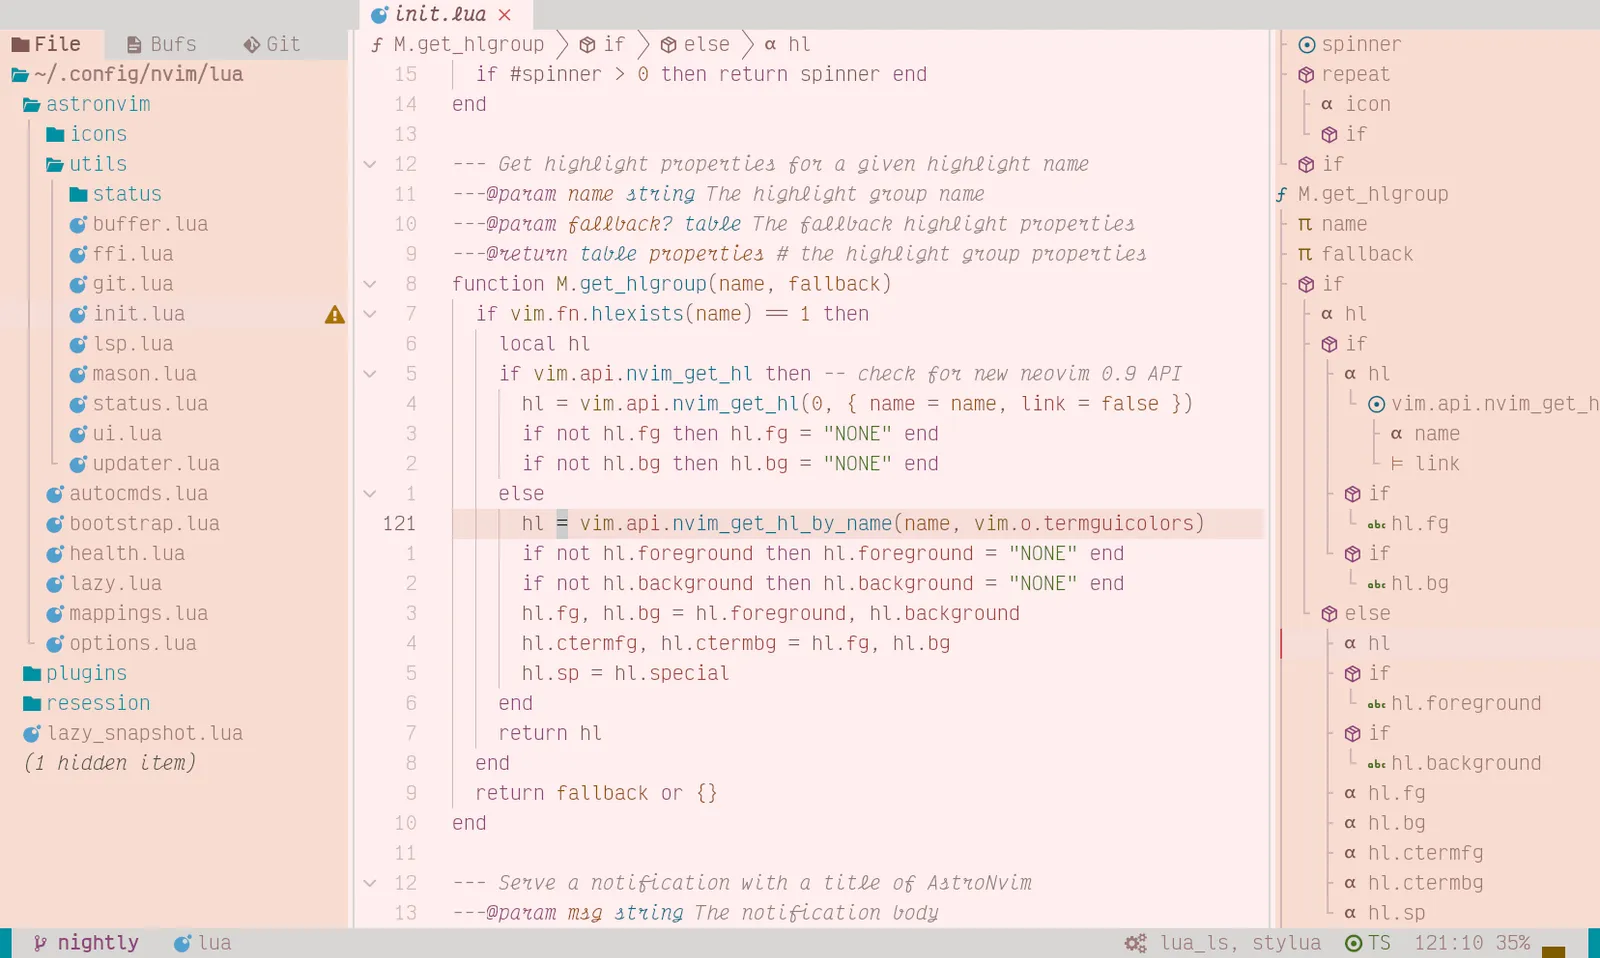
\includegraphics[width=0.8\textwidth]{astronvim_welcome.png}
    \caption{AstroNvim 界面}
    \label{fig:astronvim}
\end{figure}

\textbf{上手要点}

\begin{itemize}
\item Leader 键是空格：按下 \texttt{<Space>} 稍等片刻会弹出快捷键菜单，忘了按键组合也不用背，跟着菜单按就行；
\item \texttt{<Space>ff} 模糊搜索并打开文件，\texttt{<Space>fw} 在整个项目中搜索文字（依赖 ripgrep）；
\item 使用 \texttt{:LspInstall clangd} 安装 C++ 的语言服务器后，即可获得代码补全和跳转。
\end{itemize}

\begin{note}
界面中的图标和 zsh 的 p10k 主题一样依赖 Nerd Font，装过 MesloLGS NF 的话直接通用（见第\ref{sec:zsh-customize}节）。更多用法见官方文档：\url{https://docs.astronvim.com/}
\end{note}

\begin{exercise}\label{ex:v1-astronvim}
完成 AstroNvim 的安装，用 \texttt{<Space>ff} 打开任意一个文本文件，再用 \texttt{<Space>fw} 在某个项目目录中搜索一个关键词，体验模糊搜索。
\end{exercise}
